\clearpage


\section{Motivation and Main Objective\label{Motivation_and_Objectives}}
In general, there is a mismatch between the daily energy generation profile of PV cells and the daily energy consumption profile of a BS, as seen in Figure \ref{bs}. The profiles in Figure \ref{bs} are given as an example in this paragraph. Many different types of energy generation profiles, and energy consumption profiles typical for PV cells, and typical for BSs will be evaluated in the following chapters, respectively. 

The objective of this thesis is to develop a method to shift the surplus energy (green color area in Figure \ref{bs}) to the deficit period (gray color area in Figure \ref{bs}). This thesis will derive a new methodology based on orientation angle optimization to adjust the solar energy supply to meet the energy demand of the
BS in the time domain (black arrow in Figure \ref{bs}). This is the main objective of this thesis and will be presented in Chapter \ref{Chapter_1}. 


\begin{figure}[H]
	\centering
		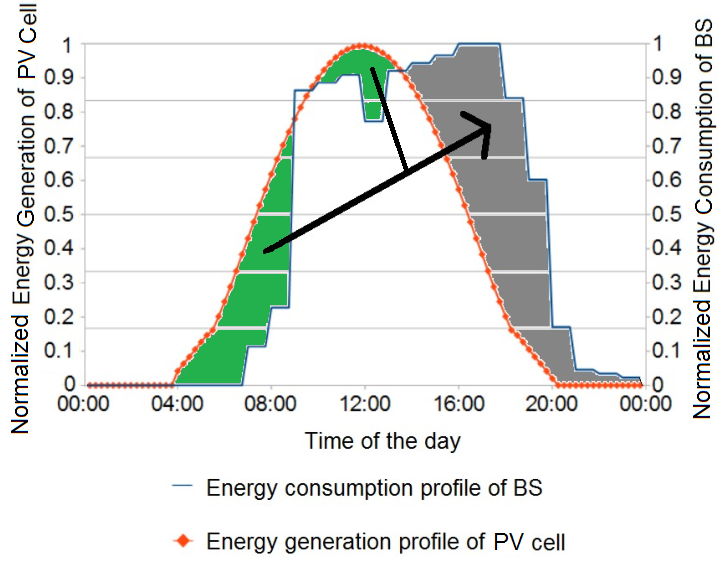
\includegraphics[width=0.7\columnwidth]{pictures/bs}
\caption{Example of an energy generation profile of a PV cell and an energy consumption profile of a BS to illustrate their mismatch\label{bs}}
\end{figure}



\clearpage
\section{Contributions\label{contributions}}
This section will summarize the main contributions of Chapter \ref{Chapter_1}, Chapter \ref{Chapter_2}, and Chapter \ref{Chapter_3}.


Contributions of Chapter \ref{Chapter_1}:

\begin{itemize}
\item Developing an algorithm to jointly optimize the orientation angles of several PV cells powering one BS. The algorithm achieves the best possible match between the energy generation profiles of the PV cells and the energy consumption profile of the BS. The proposed optimization algorithm only needs to be run a single time offline and the obtained optimal angles can be used for all solar-powered BSs with similar geographic locations and energy consumption profiles.
\item Deriving analytically the irradiance values on any randomly inclined and oriented PV cell. A horizontally-mounted PV cell is used as a baseline and its irradiance values have to be given to derive the irradiance values on any randomly inclined and oriented PV cell at the same location.
\item Identifying and discussing analytically to what extent the orientation angle $\theta$ shifts the energy generation profile away from noon if the PV cells are not south-oriented ($\theta \neq 0^\mathrm{o}$).  
\item Evaluating the effectiveness of the proposed orientation angle optimization on three different types of BS energy consumption profiles: constant traffic load profiles, business-area traffic load profiles, and residential-area traffic load profiles. The energy drawn from the main grid by the BS per day is used as the performance metric.
\item Giving recommendations on how many differently oriented PV cells should be deployed for a given energy consumption profile. To the best of my knowledge, this has never been investigated in the literature before.
\end{itemize}


Contributions of Chapter \ref{Chapter_2}:



\begin {itemize}
\item Developing a PV cell’s orientation angle optimization algorithm with Markov chain based battery model of a solar-powered BS with battery. The algorithm takes into account the battery capacity and the energy consumption profile of the BS. The number of user equipments (UEs) served by the BS throughout the day $\overline{S_{\mathrm{UE}}}(\theta)$ is used as the performance metric to identify the optimal orientation angle.
\item Verifying the accuracy of the proposed algorithm by showing that simulation trials converge based on the law of large numbers to 
the output $\overline{S_{\mathrm{UE}}}(\theta)$ of the proposed algorithm. 
\item Showing that the proposed algorithm (depends on the number of battery states) requires a shorter running time than the simulation trials (depends on the number of trials) for moderate battery state resolutions.
\item Investigating the dependency of the optimal PV cell orientation angle on the given battery capacity.
\end {itemize}


Contributions of Chapter \ref{Chapter_3}:


\begin{itemize}
\item  Developing an optimization algorithm that can be run once during the cellular network planning to determine what type of energy harvesters should be deployed to every BS in a cellular network. There are two different types of energy harvesters available for deployment which have anti-correlated energy generation profiles.
\item Taking into account the topology of the cellular network as well as the distance-dependent power loss in the distribution lines during the optimization.
\item Developing an optimization objective that maximizes the power that can be transmitted from surplus BSs to deficit BSs in the cellular network.
\item Comparing the proposed optimization algorithm with randomly deploying anti-correlated energy harvesters to the BSs. The effects of different numbers of BSs, different distribution line existence probabilities, different distribution line power loss coefficients, and different power surplus values are investigated. 
\end{itemize}





\clearpage
\section{Organization\label{Organization}}
This section will present the organization of the thesis in detail. Section \ref{back} gives a general overview of the developments and emerging problems in future cellular networks and how solar-powered BSs can alleviate these emerging issues. Section \ref{def_an} defines the orientation and inclination angles of the PV cells and provides a basic rule of thumb how these angles should be chosen based on the geographical location of the PV cell. This rule of thumb only maximizes the yearly energy output of the PV cell but it cannot take into account the energy consumption profile of the appliance. Section \ref{type_pv} justifies the focus on fixed PV cells with respect to other types of PV cells in this thesis. Section \ref{Motivation_and_Objectives}, Section \ref{contributions}, and Section \ref{Organization} present the main objectives, the contributions, and the organization of this thesis, respectively. Chapter \ref{Chapter_1}, Chapter \ref{Chapter_2}, and Chapter \ref{Chapter_3} are the main parts of this thesis and are based on my published papers. Each of the three chapters develops a system model to address and to evaluate a specific problem explained in more detail later. Guidelines and key findings are summarized at the end of each chapter.

Chapter \ref{Chapter_1} addresses the main objective of this thesis. It develops a methodology to jointly optimize the orientation angles of several PV cells at one BS so that the energy generation profile of the PV cells matches the energy consumption profile of the BS. The system model of this chapter is presented in Section \ref{system_1} and consists of an energy generation model, a ground-reflected irradiance model, a direct-beam irradiance model, a sky-diffuse irradiance model, an energy consumption model, and an objective function. Section \ref{analytical} evaluates analytically to what extent the orientation angle $\theta$ determines the position of the peak of the energy generation profile in the time domain. The numerical results and the key findings are presented in Section \ref{results}. Finally, the chapter is summarized in Section \ref{sum_Chapter_1}.



Chapter \ref{Chapter_2} extends the system model from Chapter \ref{Chapter_1} by adding a battery to the BS. The battery is modeled by a Markov chain. Section \ref{system_2} presents the system model of this chapter. Section \ref{jj} derives the PV cell's orientation angle optimization algorithm with Markov chain based battery model of a solar-powered BS with battery. Section \ref{see} introduces a simulation algorithm as a baseline for the comparison and evaluation of the proposed algorithm. Section \ref{results_system_2} discusses and presents numerical results. In more detail, Section \ref{n} investigates the running time of both algorithms. Section \ref{anna} verifies the accuracy of the proposed algorithm with simulation results.
Section \ref{new} shows the strong dependency of the optimal PV cell orientation angle on the battery capacity. Finally, the chapter is summarized in Section \ref{sum_Chapter_2}. 

Chapter \ref{Chapter_3} extends the previous system model to a multi-cell cellular network. There are now several BSs distributed in an area and some of them are connected by distribution lines to share the renewable energy among them. The problem investigated in this chapter is how energy harvesters with anti-correlated energy generation profiles should be deployed to every BS so that the renewable energy can be shared most efficiently in the multi-cell cellular network. Two PV cells that have significantly different orientation angles, such as east-oriented and west-oriented PV cells, are an example for energy harvesters with anti-correlated energy generation profiles. Section \ref{system_model_3} presents the system model of this chapter, which consists of the definition of the power surplus/deficit values, the derivation of the distance-dependent power loss in the distribution lines, and the definition of the topology of the cellular network. The objective function of this chapter is derived in Section \ref{MILPP_pres} and based on a mixed-integer linear programming problem (MILPP). Section \ref{numeric_results_system_3} presents the system performance improvements achieved by optimizing the deployment of the energy-harvesters with the MILPP in comparison with randomly deploying the energy harvesters. Finally, the chapter is summarized in Section \ref{sum_Chapter_3}.
 
Chapter \ref{conclusion} concludes the thesis by summarizing its achievements, highlighting future application areas, and outlining future work in this area. 
An appendix and a list of references are attached at the end of this thesis.








